\documentclass[11pt,a4paper]{article}
\usepackage{ngerman}
\usepackage[ngerman]{babel}
\usepackage[utf8x]{inputenc}
\usepackage[T1]{fontenc}
\usepackage{lmodern}
\usepackage{marvosym}
\usepackage{amsfonts,amsmath,amssymb}
\usepackage{textcomp}
\usepackage{pifont}
\usepackage{ifpdf}
\usepackage[pdftex]{color}
\ifpdf
  \usepackage[pdftex]{graphicx}
\else
  \usepackage[dvips]{graphicx}\fi

\pagestyle{empty}

\usepackage[scale=0.775]{geometry}
\setlength{\parindent}{0pt}
\addtolength{\parskip}{6pt}

\def\firstname{Pascal}
\def\familyname{Bernhard}
\def\FileAuthor{\firstname~\familyname}
\def\FileTitle{\firstname~\familyname's Reformation}
\def\FileSubject{Reformation}
\def\FileKeyWords{\firstname~\familyname, Reformation}

\renewcommand{\ttdefault}{pcr}
\hyphenation{ins-be-son-de-re}
\usepackage{url}
\urlstyle{tt}
\ifpdf
  \usepackage[pdftex,pdfborder=0,breaklinks,baseurl=http://,pdfpagemode=None,pdfstartview=XYZ,pdfstartpage=1]{hyperref}
  \hypersetup{
    pdfauthor   = \FileAuthor,%
    pdftitle    = \FileTitle,%
    pdfsubject  = \FileSubject,%
    pdfkeywords = \FileKeyWords,%
    pdfcreator  = \LaTeX,%
    pdfproducer = \LaTeX}
\else
  \usepackage[dvips]{hyperref}
\fi

\definecolor{firstnamecolor}{RGB}{56,115,179}
\definecolor{familynamecolor}{RGB}{56,115,179}
\hypersetup{pdfborder=0 0 0}

% Gleiche Schriftart für Hyperlinks
\urlstyle{same}


%  Gefrickel um URL-Links vernünftig umzubrechen
\makeatletter
\g@addto@macro\UrlBreaks{
  \do\a\do\b\do\c\do\d\do\e\do\f\do\g\do\h\do\i\do\j
  \do\k\do\l\do\m\do\n\do\o\do\p\do\q\do\r\do\s\do\t
  \do\u\do\v\do\w\do\x\do\y\do\z\do\&\do\1\do\2\do\3
  \do\4\do\5\do\6\do\7\do\8\do\9\do\0}
% \def\do@url@hyp{\do\-}

% Hiermit soll einer übervolle Box verhindert werden -- funktioniert sogar irgendwie
\g@addto@macro\UrlSpecials{\do\/{\mbox{\UrlFont/}\hskip 0pt plus 1pt}}
\makeatother

% Farben werden hier definiert
\definecolor{MidnightBlue}{RGB}{0,103,149}


\begin{document}
\sffamily   % for use with a résumé using sans serif fonts;
%\rmfamily  % for use with a résumé using serif fonts;
\hfill%
\begin{minipage}[t]{.6\textwidth}
\raggedleft%
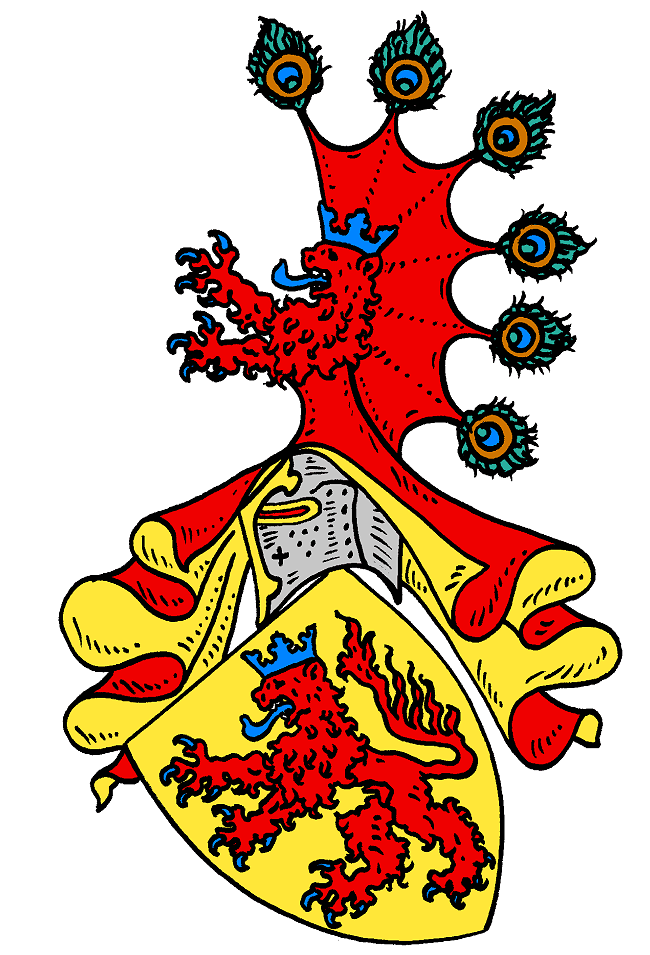
\includegraphics[width=0.55\textwidth]{Habsburg-Stammwappen.png}


%	{\bfseries {\color{firstnamecolor}\firstname}~{\color{familynamecolor}\familyname}}\\[.35ex]
%	\small\itshape%
%	Schwalbacher Straße 7\\
%	12161 Berlin\\[.35ex]
%	\Mobilefone~+49 162 32 39 557 \\
%	\Letter~\href{mailto:pascal.bernhard@rppr.de}{pascal.bernhard@rppr.de}
\end{minipage}\\[0.5em]
%
{\color{firstnamecolor}\rule{\textwidth}{.25ex}}
%
\begin{minipage}[t]{.4\textwidth}
	\raggedright%
	% {\bfseries {\color{firstnamecolor}
	\vspace*{1em}
%	\textbf{Geschichte der Habsburger -- Flaggen} \\
%	 \\[.35ex]
	% }}
	\small%
%	Wolframstraße 89-92\\
%	12105 Berlin
\end{minipage}
%
\hfill
%
\begin{minipage}[t]{.4\textwidth}
	\raggedleft % US style
	\today
	%April 6, 2006 % US informal style
	%05/04/2006 % UK formal style
\end{minipage}\\[2.2em]


{\bfseries \color{familynamecolor}{{\LARGE Die Habsburger Dynastie -- Flaggen}}}\\[0.75em]

\section*{\textsf{Die Geschichte der Habsburger}}

\begin{itemize}
\item Name der Habsburger-Dynastie leitet sich von ihrer Stammburg, der 'Habsburg' im Schweizer Kanton \textsl{Aargau} ab
\item Fürstengeschlecht geht auf den Grafen \textsl{Guntram der Reiche} (\textdied973), der Landbesitz am Oberrhein hatte


\item um 1027 gründete der direkte Nachfahre Radbot (945-1045) mit seiner Ehefrau Ita von Lothringen (995-1035) das Benediktinerkloster \textsl{Muri} im Kanton Aargau

\item als Mittelpunkt der Herrschaft der Fürsten wurde die Habsburg um 1020 errichtet

\item Otto, Graf von Habsburg (\textdied1111) war das erste Familienmitglied, welches sich 'von Habsburg' nannte

\end{itemize}

\subsection*{\textsf{Aufstieg der Habsburger zu einer europäischen Dynastie}}

\begin{itemize}
\item Rudolf IV konnte seinen Herrschaftsraum im späten 13.Jahrhundert systematisch ausbauen\\
\ding{225} Ländereien im Schwarzwald und Herrschaft über die Ost- \& Nordschweiz\\
\ding{225} Krönung zum römisch-deutschen König 1273 (damals gab es noch nicht die Bezeichnung Kaiser) als Rudolf I

\item ab 1278 begann die Herrschaft der Habsburger im heutigen Österreich (Nieder- \& Oberösterreich sowie der Steiermark)\\
\ding{225} Belehnung der Söhne Rudolfs mit den Ländereien der Babenberger, den Herzogtümern Österreich und Steiermark

\item Verlust der Schweizer Territorien im 14. und 15.Jahrhundert -- die Habsburg fällt 1415 an die Eidgenossen\\
\ding{225} Machtzentrum der Habsburger verlagert sich nach Osten

\item nachdem er in der \textsl{Goldenen Bulle} nicht als Kurfürst des Heiligen Römischen Reiches berücksichtigt worden war, ließ Rudolf IV eine kaiserliche Urkunde fälschen, die den Österreichischen Stammlanden der Habsburger umfangreiche Rechte (Unteilbarkeit der Länder, eigene Gerichtsbarkeit, automatische Erbfolge, eigene Symbole) zustand und sie als Erzherzogtum deklarierte\\
\ding{225} Urkunde wurde vom damaligen römisch-deutschen Kaiser Friedrich III anerkannt

\item seit der Wahl Albrechts II im Jahre 1438 zum Deutschen Kaiser stellten die Habsburger (mit Ausnahme Kaisers Karls VII 1742-1745) alle Kaiser des Heiligen Römischen Reiches Deutscher Nation

\item durch geschickte Heiratspolitik erwarben die Habsburger Ende des 15. Jahrhunderts die Niederlande, die Freigrafschaft Burgund und darauffolgend die Kronen Böhmens, Spaniens, Kroatien und Ungarns

\item Höhepunkt des Habsburger Reiches mit Karl V, in dessen Weltreich "`die Sonne nie unterging"'

\end{itemize}



\subsection*{\textsf{Die Habsburger in der modernen Neuzeit}}

\begin{itemize}
\item nach dem Tod Karls V teilte sich die Dynastie in einer spanische und eine österreichische Linie

\item im Jahre 1740 gab es nach dem Tod Karls VI für die österreichische Linie der Habsburger keinen männlichen Thronfolger\\
\ding{225} seine Tochter Maria Theresia übernahm durch eine Sonderregelung im Erbrecht (bereits 1713 vorgenommen) die Herrschaftsrechte

\item nach der Hochzeit Maria Theresias mit Franz Stephan von Lothringen nannte sich die Dynastie \textsl{Habsburg-Lothringen}

\end{itemize}


\subsection*{\textsf{Kaisertum Österreich}}

\begin{itemize}

\item vor der Schlacht von Austerlitz hatte der damalige König Östereichs Franz II sich zum Kaiser Franz I ausgerufen, um Ranggleichheit mit Napoleon und dem russischen Zaren zu haben\\
\ding{225} \textsl{Drei-Kaiser Schlacht}

\item nach Druck des ungarischen Adels wurde das Kaisertum Österreich in die Österreichisch-Ungarische Monarchie umgewandelt\\
\ding{225} der österreichische Kaiser war zugleich König Ungarns\\
\ding{225} K.u.K Monarchie -- Kaiser und König Monarchie

\item am 11. November 1918 verzichtet Kaiser Karl I auf alle Staatsgeschäfte\\
\ding{225} keine formale Abdankung\\
\ding{225} kaiserliche Familie floh 1919 in die Schweiz, um einer Verhaftung zu entgehen


\end{itemize}

\section*{\textsf{Flaggen der Österreichs, Deutschlands und der Schweiz}}


\subsection*{\textsf{Schweizer Flagge}}

\begin{itemize}

\item die Schweizer Flagge geht auf die Zeit der Eidgenössischen Kriege zurück

\item jeder Kanton führte im Krieg seine eigene Fahne mit sich, eine Schweizer Fahne gab es in der damaligen Zeit noch nicht

\item die Soldaten des Kantons Schwyz hatten eine rote Flagge und durften seit ihrer Unterstützung Rudolfs IV von Habsburg im Krieg gegen Burgund das weiße Kreuz als Symbol der Kreuzigung Christi hinzufügen

\item je größer die Eidgenossenschaft wurde, desto schwieriger wurde es, die Soldaten der vielzähligen Kantone voneinander zu unterscheiden\\
\ding{225} das weiße Kreuz wurde zum gemeinsamen Erkennungszeichen

\item das Schweizer Kreuz mit seinen gleichen Seitenverhältnissen war zugleich eine Abgrenzung der Schweizer Söldner gegen das Andreaskreuz der deutschen Landsknechte


\end{itemize}



\subsection*{\textsf{Flagge Österreichs}}

\begin{itemize}

\item die Farben Rot-Weiß-Rot der österreichischen Fahne geht auf das Schild des Adelsgeschlechts der Babenberger zurück

\item nachdem die Habsburger 1270 mit den Besitzungen der Babenberger belehnt wurden, integrierten sie dessen Farben in das eigene Wappen

\item ab dem 15. Jahrhundert wurde Rot-Weiß-Rot endgültig zum Wappen Österreichs


\end{itemize}



\subsection*{\textsf{Deutsche Flagge}}


\begin{itemize}

\item Vorläufer der Kombination Schwarz-Rot-Gold war das Reichsbanner der Heiligen Römischen Reiches Deutscher Nation (Schwarzer Adler mit roten Krallen auf goldenem Grund)

\item die moderne deutsche Fahne aus Schwarz-Rot-Gold hat seinen Ursprung in den Befreiungskriegen 1813 gegen Napoleon\\
\ding{225} die Freiwilligen des Lützowschen Freikorps setzte sich vor allem aus Studenten mit unterschiedlichster Kleidung zusammen\\
\ding{225} alle Bekleidung wurde schwarz gefärbt und goldene Messingknöpfe sowie rote Kragen und Aufschläge aufgenäht\\
\ding{225} aus diesem Freikorps gründete sich die 'Urburschenschaft', die Schwarz-Rot-Gold zu ihrer Fahne wählten\\
\ding{225} Wahlspruch: \textsl{Aus der Schwärze (schwarz) der Knechtschaft durch blutige (rot) Schlachten ans goldene (gold) Licht der Freiheit}

\item am vierten Jahrestag der Völkerschlacht von Leipzig zog die Urburschenschaft unter der 'Deutschen Flagge' und der Losung 'Nur im Ganzen heil' auf die Wartburg

\item die Farben Schwarz-Rot-Gold wurden zur Zeit des Deutschen Bundes (1815-1866) zu den deutschen Nationalfarben

\item die Revolutionäre, welche die Einheit Deutschlands als Republik und nichts als Monarchie forderten, nahmen die dreifarbige Fahne in Anlehnung an die französische Trikolore

\item nach Ende des Kaiserreiches wurde von der Weimarer Republik Schwarz-Rot-Gold als nationales Flagge gewählt


\end{itemize}



\end{document}